\section{Задание 2. Исследование функции двух переменных}

\textbf{Условие.}

\begin{enumerate}[label=\Alph*.]
    \item Изобразите поверхность, заданную уравнением $z=z(x,y)$, в программе Geogebra 3D.

    Выполните следующие этапы исследования:

    \begin{enumerate}[label=\arabic*.]
        \item Найдите область определения $z = z(x, y)$.

        \item Постройте в программе Geogebra Classic (на одном листе!) семейство линий уровня $z(x, y) = c$.
        Для построения выберите 3–4 значения $c$.
        Определите тип построенных кривых (найдите уравнения линий уровня при выбранных значениях $c$).
        Если разным $c$ соответствуют кривые разных типов (например: прямые, окружности, точка), изобразите все типы линий уровня.

        \item Выберите на поверхности какую-либо обыкновенную и не стационарную точку $M_0$ (определите ее координаты $x_0, y_0, z = z(x_0, y_0)$).
        Докажите (по определению), что выбранная точка не является особой и стационарной.

        \item Найдите вектор $\overrightarrow{m}$ - направление наискорейшего спуска (подъема) в точке $M_0$.

        \item Изобразите в программе Geogebra Classic линию уровня $z = z(x_0, y_0)$ и направление.
        Проверьте их ортогональность.

    \end{enumerate}

    \item Найдите наибольшее и наименьшее значения функции $u = u(x, y)$ в области $D$:

    \begin{enumerate}[label=\arabic*.]
        \item Найдите стационарные точки внутри области.
        \item Определите, являются ли стационарные точки точками экстремума.
        \item Исследуйте значения функции вдоль границ области.
        \item Определите точки области, в которых достигаются наибольшее и наименьшее значения функции, и сами значения
    \end{enumerate}

    \vspace{5mm}

    \begin{tabular}{ccc}
        Функция $z = z(x, y)$                     & Функция $u = u(x, y)$         & Область $D$                          \\
        $\displaystyle z = \frac{8y}{x^2 + 4y^2}$ & $u = x^2 + 2x + y^2 - 4y + 4$ & $0 \leq x \leq 2, \ 0 \leq y \leq 3$
    \end{tabular}
\end{enumerate}

\vspace{10mm}
\textbf{Решение.}

\begin{enumerate}[label=\Alph*.]
    \item Изображение данной поверхности $\displaystyle z = \frac{8y}{x^2 + 4y^2}$

    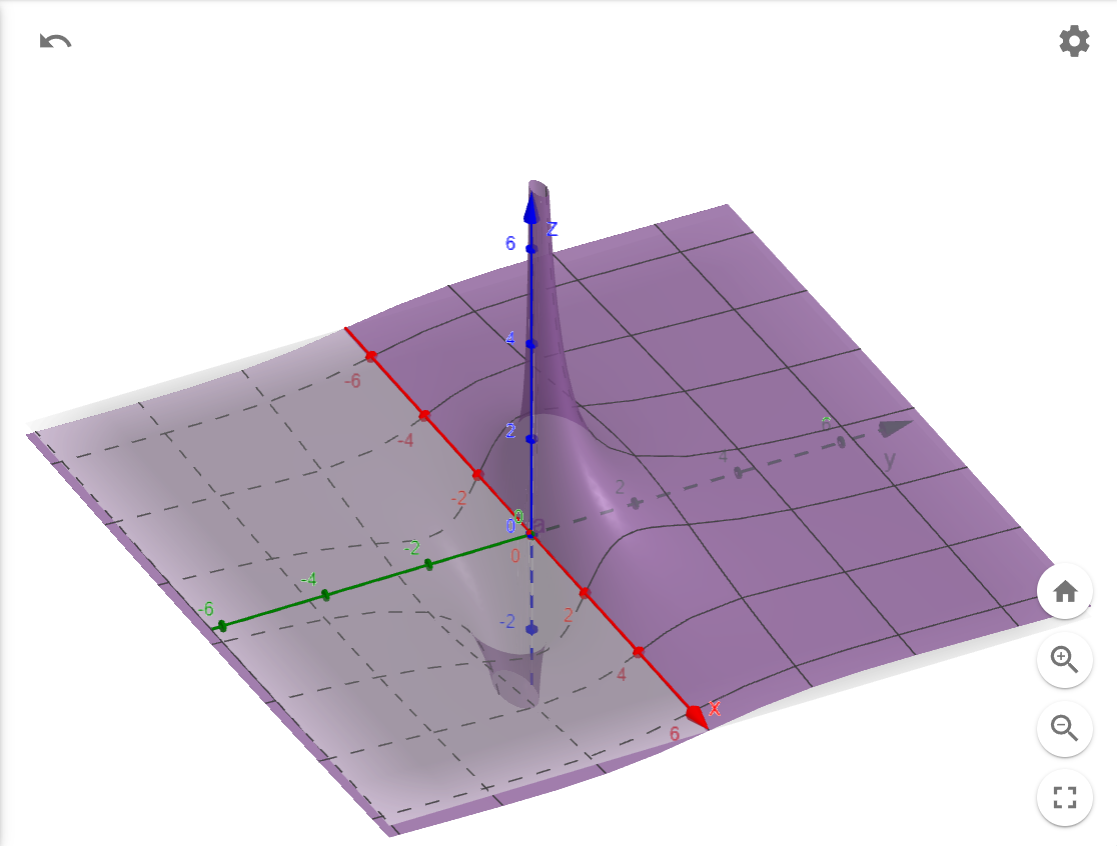
\includegraphics[height=60mm]{images/2a1}

    \begin{enumerate}[label=\arabic*.]
        \item Исследуем $\displaystyle z = \frac{8y}{x^2 + 4y^2}$ - функция принимает все значения $(x, y)$, кроме тех,
        что дают нулевой знаменатель, то есть $x^2 + 4y^2 = 0 \Longrightarrow x = y = 0$

        $D(z) = \Real^2 \setminus \Set{(0, 0)}$

        \item Заметим, что при $z = 0$ получаем $\displaystyle \frac{8y}{x^2 + 4y^2} = 0 \Longrightarrow y = 0 (x \neq 0)$ - прямую с выколотой точкой

        При $z > 0$ получаем $\displaystyle zx^2 + 4zy^2 = 8y \Longrightarrow
        zx^2 + 4zy^2 - 8\frac{\sqrt{z}}{\sqrt{z}}y + \frac{4}{z} - \frac{4}{z} = 0 \Longrightarrow \\
        zx^2 + \left(2\sqrt{z}y - \frac{2}{\sqrt{z}}\right)^2 = \frac{4}{z}$ - эллипс

        Аналогично при $z < 0$ получаем $\displaystyle zx^2 - \left(2\sqrt{|z|}y + \frac{2}{\sqrt{|z|}}\right)^2 = -\frac{4}{z}$ - эллипс

        Возьмем кривые при $z = 0, z = 3, z = -1$, вот, как они будут выглядеть:

        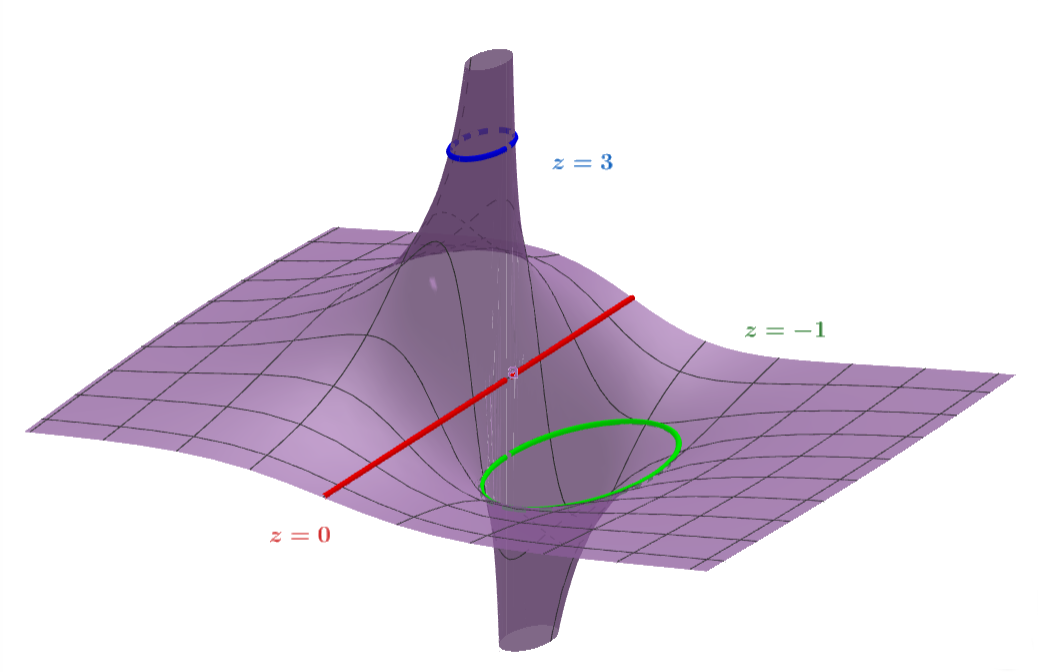
\includegraphics[height=70mm]{images/2a2}

        \item Выберем точку $M_0 = (1, 0, 0)$. Она нестационарная, по определению стационарные точки - это те, в которых

        $\begin{cases}
             \frac{\partial z}{\partial x} = \frac{16xy}{(x^2 + 4y^2)^2} = 0 \\
             \frac{\partial z}{\partial y} = \frac{8x^2 + 32y^2 - 64y^2}{(x^2 + 4y^2)^2} = 0
        \end{cases}$

        Но простой подстановкой мы можем убедиться, что это не так.

        Она обыкновенная: пусть наша поверхность - $\displaystyle F(x, y, z) = z - \frac{8y}{x^2 + 4y^2} = 0$,
        тогда по определению особой точки должна выполняться система:

        $\begin{cases}
             \frac{\partial F}{\partial x} = -\frac{16xy}{(x^2 + 4y^2)^2} = 0 \\
             \frac{\partial F}{\partial y} = -\frac{8x^2 + 32y^2 - 64y^2}{(x^2 + 4y^2)^2} = 0 \\
             \frac{\partial F}{\partial z} = 0 \\
        \end{cases}$

        Но это не выполняется, так как $\displaystyle \frac{\partial F}{\partial z} = 1 \neq 0$


        \item Найдем вектор направления наискорейшего подъема при помощи градиента:

        $\overrightarrow{m} = \overrightarrow{\triangledown} F = \left(-\frac{16xy}{(x^2 + 4y^2)^2}\overrightarrow{i} - \frac{8x^2 + 32y^2 - 64y^2}{(x^2 + 4y^2)^2}\overrightarrow{j} + \overrightarrow{k}\right) \Big|_{M_0} =
        -8\overrightarrow{j} + \overrightarrow{k}$

        \item В точке $M_0$ линии уровня $z = z(M_0) = 0$ - это $y = 0 (x \neq 0)$ с направляющим вектором $(1, 0, 0)$.

        Вектор направления $\overrightarrow{m}$ в точке $M_0$ - это $(0, -8, 1)$

        Их скалярное произведение $(1, 0, 0) \cdot (0, -8, 1) = 0$ - линия уровня $z = 0$ и $\overrightarrow{m}$ перпендикулярны

        Вот изображение линии уровня и вектора $\overrightarrow{m}$:

        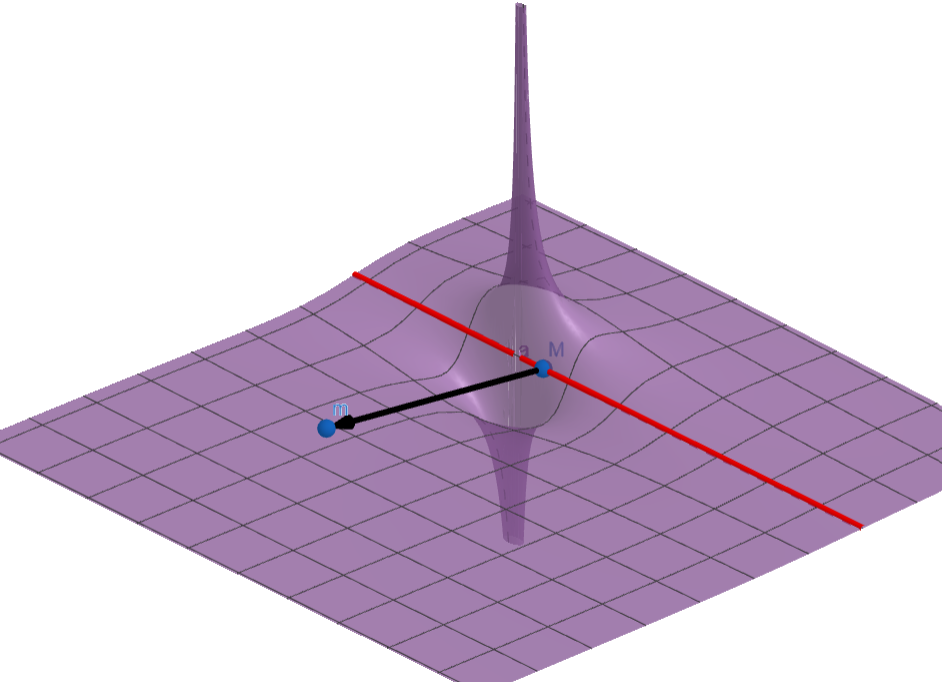
\includegraphics[height=60mm]{images/2a3}
    \end{enumerate}

    \item Найдем наибольшее и наименьшее значения функции $u = x^2 + 2x + y^2 - 4y + 4$ в области $D \{0 \leq x \leq 2, \ 0 \leq y \leq 3\}$:

    \begin{enumerate}[label=\arabic*.]
        \item По определению стационарные точки - это те, в которых выполняется система:

        $\begin{cases}
             \frac{\partial u}{\partial x} = 2x + 2 = 0 \\
             \frac{\partial u}{\partial y} = 2y - 4 = 0
        \end{cases} \Longrightarrow \begin{cases}
                                        x = -1 \\
                                        y = 2
        \end{cases}$

        \item Найдем производные второго порядка:

        $A = \frac{\partial^2 u}{\partial x^2} = 2; B = \frac{\partial^2 u}{\partial x \partial y} = 0; C = \frac{\partial^2 u}{\partial y^2} = 2$

        По достаточному условию экстремума в точке должно соблюдаться $AC - B^2 > 0$, что в точке $(-1, 2)$ верно, поэтому она экстремум

        \item Приведем график этой функции и ее значений в данной области:

        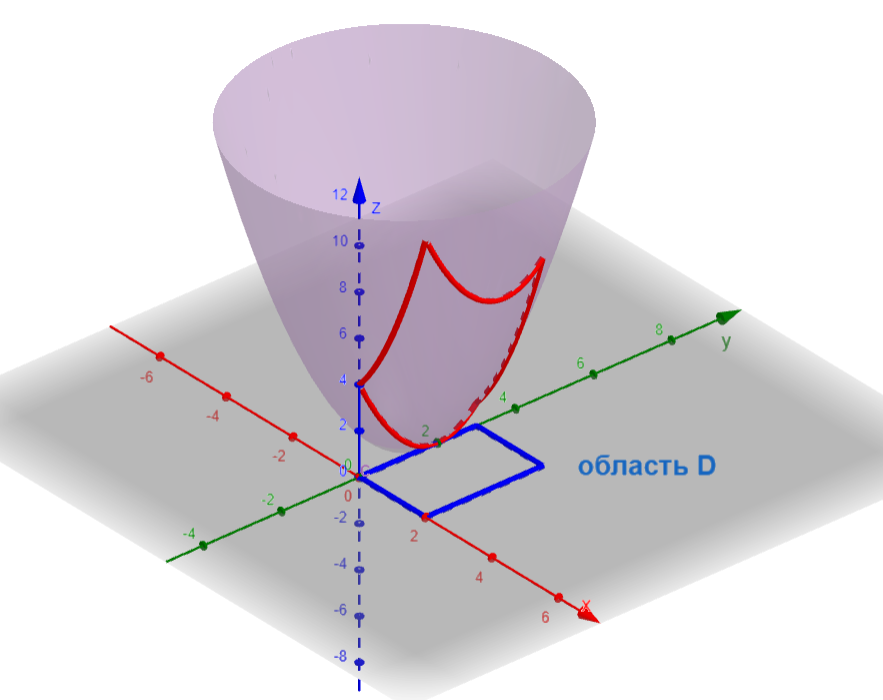
\includegraphics[height=60mm]{images/2b1}

        Как можем заметить, все значения в данной области неотрицательные

        \item Исходя из графика выше, наименьшее значения в области $D$ достигается в точке $(0, 2)$ - это $0$

        Так как, функция - это эллипсоидный параболоид (в данном случае эллипс - это окружность), то наибольшее значение
        этой функций будет достигаться при наибольшем удалении от центра параболоида (что в нашем случае минимум параболоида, то есть $(-1, 2)$)

        Таким образом, из всех точек в области подходит точка $(2, 0)$, находящаяся от центра на расстоянии $\sqrt{13}$,
        а функция в данной точке имеет значение $12$

        Аналогично находится минимум: точка $(0, 2)$ ближайшая к центру, поэтому функция принимает в нем наименьшее значение, то есть $0$, что соответствует графику выше
    \end{enumerate}

\end{enumerate}

\clearpage
